\documentclass{report}
\usepackage{amsmath}
\usepackage{parskip}
\usepackage{pdfpages}

\begin{document}
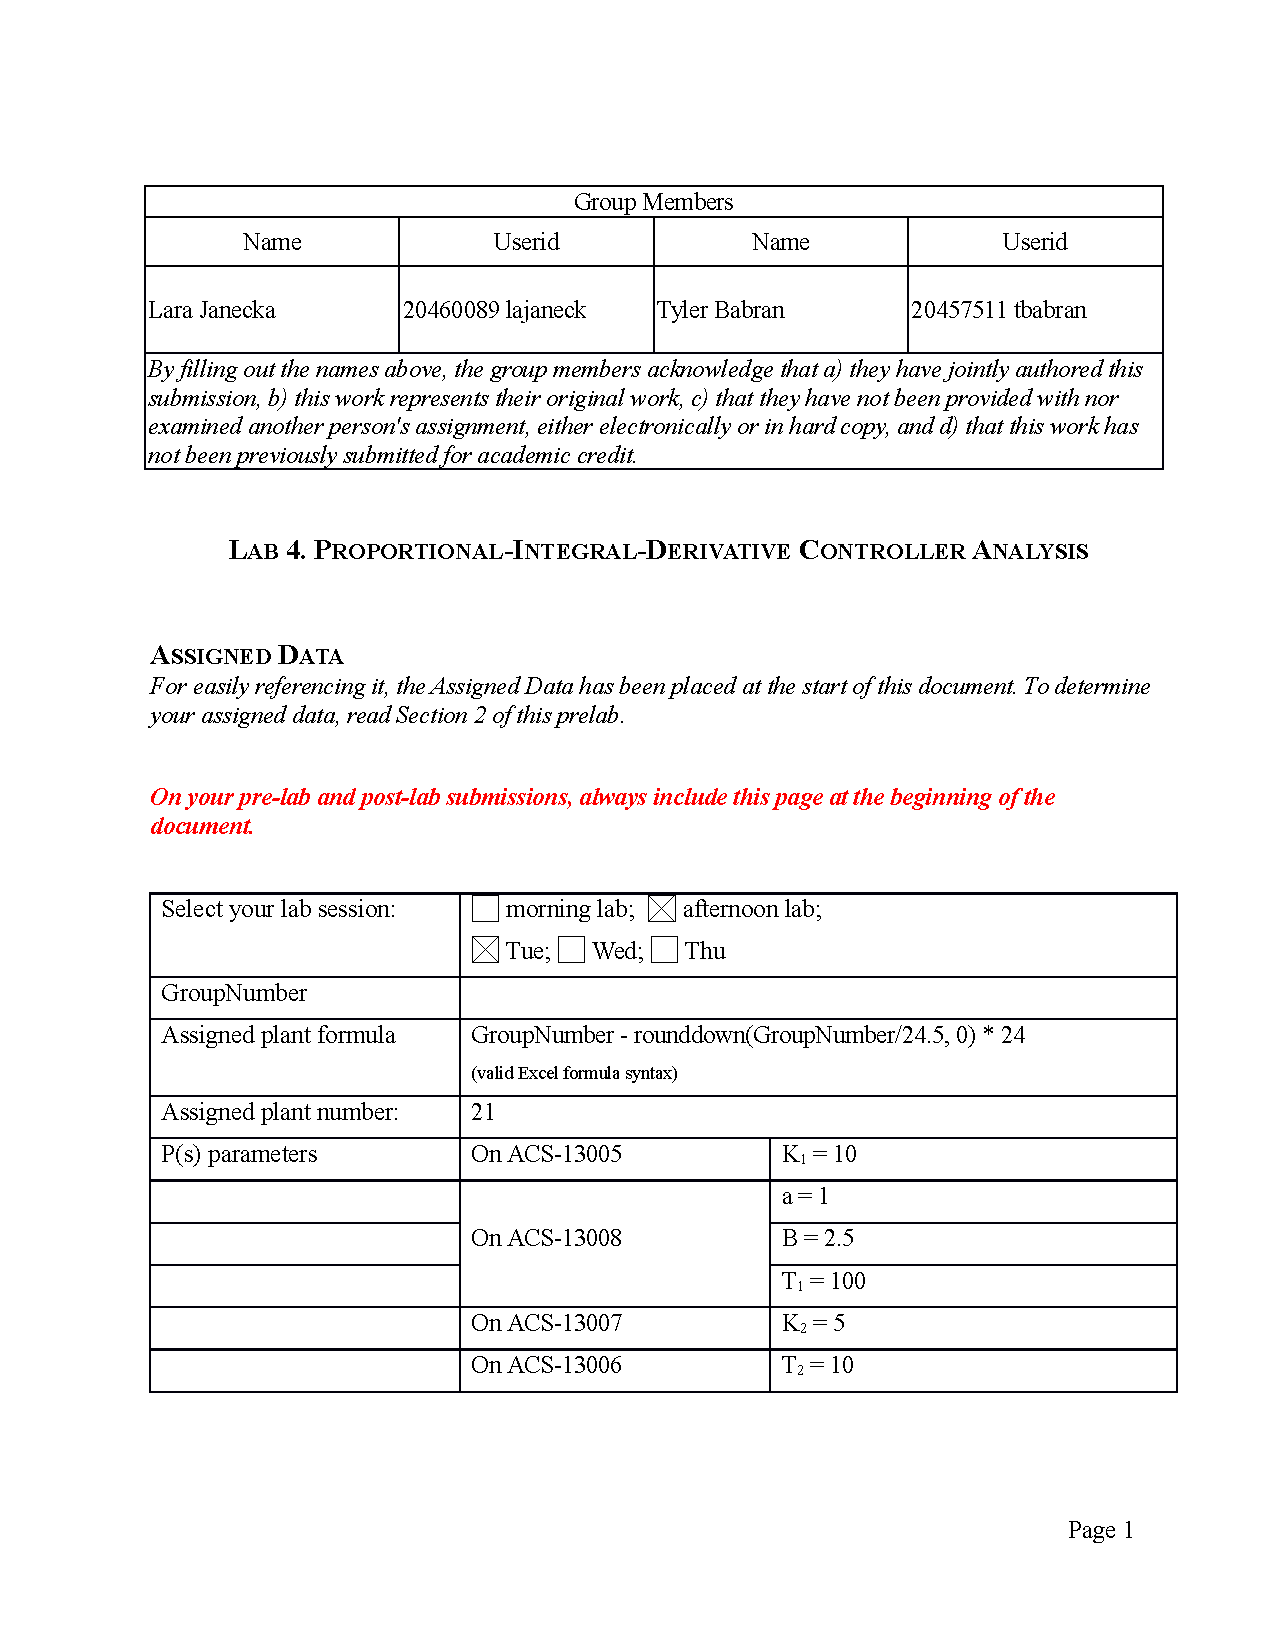
\includepdf{page1}
\section*{Prelab} % (fold)
\label{sec:pre_lab}

\subsection*{A)} % (fold)
\label{sub:a_}
\begin{align*}
    y(t) &= K * (1 -e^{-aTt})\\
    y(\frac{1}{aT}) &= K(1 -e^{-1})\\
        &= 0.63K
\end{align*}
% subsection a_ (end)

\subsection*{B)} % (fold)
\label{sub:b_}
\begin{align*}
    0.98K &= y(t)\\
        &= K(1 - e^{-aTt})\\
    1 &= 0.02e^{aTt}\\
    50 &= e^{aTt}\\
    \ln50 &= aTt\\
    t &= \frac{\ln50}{aT}
\end{align*}
% subsection b_ (end)

\subsection*{C)} % (fold)
\label{sub:c_}
\begin{align*}
    dB &= 20\log_{10}\bigg(\frac{V_{out}}{v_{in}}\bigg)\\
    dB &= 20\log_{10}\bigg|\frac{KaT}{jw + aT}\bigg|\\
    dB_{low} &= 20\log_{10}\bigg|\frac{KaT}{aT}\bigg|\\
    dB_{low} &= 20\log_{10}K
\end{align*}

\begin{align*}
    \frac{dB_{low}}{\sqrt{2}} &= 20\log_{10}\bigg|\frac{KaT}{jw_c + aT}\bigg|\\
    \frac{20\log_{10}K}{\sqrt{2}} &= 20\log_{10}\bigg|\frac{KaT}{400j + aT}\bigg|\\
    \frac{\log_{10}K}{\sqrt{2}} &= \log_{10}\bigg(\frac{KaT}{\sqrt{1600 + a^2T^2}}\bigg)\\
    10^\frac{\log_{10}K}{\sqrt{2}} &= 10^{\log_{10}(\frac{KaT}{\sqrt{1600 + a^2T^2 }})}\\
    K^{\frac{1}{\sqrt{2}}} &= \frac{KaT}{\sqrt{1600 + a^2T^2}}\\
    K^{\sqrt{2}} &= \frac{K^2a^2T^2}{1600 + a^2T^2}\\
    1600K^{\sqrt{2}} &= (K^2 - K^{\sqrt{2}})a^2T^2\\
    a^2T^2 &= \frac{1600K^{\sqrt{2}}}{K^2 - K^{\sqrt{2}}}\\
    aT &= \sqrt{\frac{1600K^{\sqrt{2}}}{K^2 - K^{\sqrt{2}}}}\\
    \text{Let K = 3}\\
    aT &= \sqrt{\frac{1600\times 3^{\sqrt{2}}}{3^2 - 3^{\sqrt{2}}}}\\
    aT &= 42.09\\
\end{align*}
Since $T$ must be \{1, 10, 100\} and $a$ must be (1,10) one possible answer is $a = 4.2$ and $T = 10$.
% subsection c_ (end)

\section*{D)} % (fold)
\label{sec:d_}
\begin{align*}
    Y(S) &= \frac{KaT}{s + aT}\\
    Y(jw_c) &= \frac{KaT}{jw_c + aT}\\
    \text{Since } \tau = \frac{1}{aT} & \text{ then } aT=\frac{1}{\tau}\\
    Y(jw_c) &= \frac{KaT}{jw_c + \frac{1}{\tau}}\\
    \frac{dB_{low}}{\sqrt{2}} &= \frac{K\frac{1}{\tau}}{jw_c + \frac{1}{\tau}}\\
    w_c &= \frac{(K-\frac{dB_{low}}{\sqrt{2}})\times\frac{1}{\tau}}{j\times\frac{dB_{low}}{\sqrt{2}}}\\
    w_c &= \frac{(K-\frac{dB_{low}}{\sqrt{2}})}{\tau \times j\times\frac{dB_{low}}{\sqrt{2}}}\\
\end{align*}
% section d_ (end)

In this system the relationship between bandwidth and time constant is a coefficient dependent on K.

\subsection*{E)} % (fold)
\label{sub:e_}
Let the signal between the ACS-13001 and ACS-13002 be called H(S).
\begin{align*}
    Y(S) &= H(S)G(S)\\
    H(S) &= R(S)-Y(S)\\
    R(S) &= H(S) + Y(S)\\
        &= H(S) + H(S)G(S)\\
    \frac{Y(S){R(S)}} &= \frac{G(S)}{1+G(S)}\\
    Y(S) &= R(S) \times \frac{G(S)}{1+G(S)}\\
        &= \frac{1}{s} \times \frac{\frac{KbT}{s + aT}}{1 + \frac{KbT}{s + aT}}\\
        &= \frac{KbT}{s(s+aT)(1 + \frac{KbT}{s + aT})}\\
        &= \frac{KbT}{s^2 + (1+K)saT}\\
\end{align*}

Now solving for the low frequency gain

\begin{align*}
    dB_{low} &= 20 \log\bigg(\frac{V_{out}}{V_{in}}\bigg)\\
        &= 20 \log\bigg|s \times \frac{KbT}{s^2 + (1+K)saT} \bigg|\\
        &= 20 \log\bigg| \frac{KbT}{s + (1+K)aT} \bigg|\\
        &= 20 \log\bigg| \frac{KbT}{jw + (1+K)aT} \bigg|\\
        \text{low frequency gain occurs at} & w=0\\
        &= 20 \log\bigg| \frac{KbT}{0+ (1+K)aT} \bigg|\\
        &= 20 \log\bigg| \frac{KbT}{(1+K)aT} \bigg|\\
        \text{Subbing in values from c) } & a=b\\
        &= 20 \log\bigg(\frac{K}{K+1}\bigg)\\
\end{align*}

Now solving for bandwidth

\begin{align*}
    \frac{dB_{low}}{\sqrt{2}} &= 20\log\bigg|\frac{KaT}{jw_c + (1+K)aT}\bigg|\\
    \frac{20 \log(\frac{K}{K+1})}{\sqrt{2}} &= 20\log\bigg|\frac{KaT}{jw_c + (1+K)aT}\bigg|\\
    \frac{\log(\frac{K}{K+1})}{\sqrt{2}} &= \log\bigg|\frac{KaT}{jw_c + (1+K)aT}\bigg|\\
    \bigg(\frac{K}{K+1}\bigg)^{\frac{1}{\sqrt{2}}} &=\bigg|\frac{KaT}{jw_c + (1+K)aT}\bigg|\\
    \bigg(\frac{K}{K+1}\bigg)^{\frac{1}{\sqrt{2}}} &=\frac{KaT}{\sqrt{w_c^2 + (1+K)^2a^2T^2}}\\
    \bigg(\frac{K}{K+1}\bigg)^{\sqrt{2}} &=\frac{K^2a^2T^2}{w_c^2 + (1+K)^2a^2T^2}\\
    \bigg(\frac{K}{K+1}\bigg)^{\sqrt{2}}w_c^2 &= K^2a^2T^2 - \bigg(\frac{K}{K+1}\bigg)^{\sqrt{2}} \times (1+K)^2a^2T^2\\
    \text{Sub in values from c)}\\
    \bigg(\frac{3}{3+1}\bigg)^{\sqrt{2}}w_c^2 &= 3^2\times 4.2^2 \times 10^2 - \bigg(\frac{3}{3+1}\bigg)^{\sqrt{2}} \times (1+3)^2 \times 4.2^2 \times 10^2\\
    w_c & = 66.16
\end{align*}

% subsection e_ (end)

% section pre_lab (end)
\end{document}
